\documentclass{article}
\usepackage[margin=1in]{geometry} % Définit la marge à 1.5 pouces
\usepackage{amsmath}
\usepackage{graphicx}
\usepackage{array} % Pour utiliser m{}
\usepackage{subcaption}
\author{Auteur : SABIDANI YENTEM ELISEE}
\title{Rapport : Analyse sémantique des images sur les maladies du manioc}
\date{\today}
\begin{document}
	
	\maketitle
	
	\newpage
	\tableofcontents
	\newpage
	

	\section{Chapitre 1 : Etat de l'art}
	\subsection{Définitions}
	\subsubsection{L'analyse sémantique des images}
	\quad L'analyse sémantique des images est un domaine de l'intelligence artificielle qui vise à comprendre le contenu visuel des images en leur attribuant des significations sémantiques. Contrairement à l'analyse basée uniquement sur des caractéristiques visuelles telles que la couleur, la texture ou la forme, l'analyse sémantique cherche à interpréter le contenu des images de manière similaire à la façon dont les humains le font.
	
	\subsubsection{Détection d'objets}
	\quad L'analyse sémantique des images comprend la détection et la reconnaissance d'objets, tels que des personnes, des animaux, des véhicules, des bâtiments, des meubles, etc. Cela implique souvent l'utilisation de réseaux de neurones convolutionnels (CNN) et de modèles d'apprentissage profond pour localiser et identifier les objets dans une image.
	
	\subsubsection{Classification}
	\quad Il s'agit d'attribuer des étiquettes ou des catégories sémantiques aux images en fonction de leur contenu. Par exemple, une image pourrait être classée comme "paysage", "portrait", "nourriture", "sport", etc. Les techniques de classification utilisent généralement des modèles de machine learning supervisés pour prédire la classe ou la catégorie d'une image.
	
	\subsubsection{Annotations d'images}
	 Les annotations d'images consistent à ajouter des métadonnées ou des informations supplémentaires à une image. Ces informations peuvent inclure des balises, des descriptions, des régions d'intérêt, des catégories, des étiquettes, etc
	 
	 \subsubsection{Méthode d'apprentissage}
	 Une méthode d'apprentissage pour la détection d'images fait référence à l'approche utilisée pour entraîner un modèle d'intelligence artificielle à reconnaître et localiser des objets dans des images.
	
	\subsubsection{Segmentation sémantique}
	\quad Au-delà de la simple détection d'objets, la segmentation sémantique vise à attribuer des étiquettes sémantiques à chaque pixel de l'image, en les regroupant en régions correspondant à des objets ou des parties d'objets spécifiques. Cela permet une compréhension fine du contenu des images et est souvent utilisé dans des domaines tels que la vision par ordinateur médicale, la conduite autonome et la réalité augmentée.
	
	\subsubsection{Reconnaissance de scènes}
	\quad Cette tâche consiste à identifier le contexte général ou la scène représentée dans une image. Par exemple, une image pourrait être reconnue comme une "feuille", une "arbre", un "forêt", etc. La reconnaissance de scènes nécessite une compréhension plus holistique du contenu de l'image et peut être réalisée à l'aide de modèles d'apprentissage automatique ou de réseaux de neurones.
	
	\subsubsection{Relation entre objets}
	\quad En plus de détecter des objets individuels, l'analyse sémantique des images peut également viser à comprendre les relations spatiales et sémantiques entre ces objets. Par exemple, une image pourrait être analysée pour déterminer si deux personnes se tiennent la main, si un objet est sur un autre, etc. Cette capacité à comprendre les relations entre objets contribue à une compréhension plus profonde du contenu visuel.\\
	
	\quad En résumé, l'analyse sémantique des images vise à extraire des informations riches et significatives à partir du contenu visuel des images, ce qui permet de mieux comprendre et d'exploiter les données visuelles dans une variété d'applications, notamment la recherche d'images, la surveillance vidéo, la médecine, l'industrie, etc.
	
	\subsubsection{Le Web sémantique}
	\quad Le Web sémantique est une extension du World Wide Web dans laquelle l'information est structurée de manière à être interprétable par les machines, permettant ainsi aux ordinateurs de comprendre le sens des données et des relations entre elles. Conçu pour rendre les contenus du Web plus intelligibles et exploitables par les machines, le Web sémantique repose sur l'utilisation de formats standardisés (comme RDF, OWL et SPARQL) pour représenter les connaissances de manière formelle et expressive. En utilisant ces standards, le Web sémantique vise à faciliter la recherche d'information avancée, l'intégration de données provenant de sources diverses, le raisonnement automatique et le développement d'applications intelligentes. En résumé, le Web sémantique vise à transformer le Web en une vaste base de connaissances interconnectée, où les données sont organisées et structurées de manière à être accessibles, compréhensibles et utilisables par les machines.
	
	\subsubsection{Rapport entre L'analyse sémantique des images et le Le Web sémantique}
	Le rapport entre le Web sémantique et l'analyse sémantique des images réside dans leur objectif commun de donner un sens aux données de manière structurée et interprétable par les machines. \\
	
	\textemdash \textbf{ Représentation des connaissances :}
	\begin{itemize}
		\item Le Web sémantique utilise des langages comme RDF et OWL pour représenter les connaissances de manière formelle et structurée.
		\item Dans l'analyse sémantique des images, les données visuelles extraites des images sont représentées de manière sémantique en utilisant des structures telles que des ontologies ou des modèles de données.
	\end{itemize}

	\textemdash \textbf{ Le Web sémantique :}
	\begin{itemize}
		\item Le Web sémantique vise à donner un sens aux données sur le World Wide Web en utilisant des standards et des technologies pour définir des relations sémantiques entre les données.
		\item l permet l'interopérabilité des données et facilite leur partage et leur intégration entre différentes sources.
	\end{itemize}

	\textemdash \textbf{ L'analyse sémantique des images :}
	\begin{itemize}
		\item L'analyse sémantique des images consiste à attribuer des significations sémantiques aux données visuelles, comme les objets, les scènes et les relations entre eux.
		\item Elle utilise les principes du Web sémantique pour interpréter le contenu des images de manière automatique et significative, permettant des applications avancées telles que la recherche d'images sémantique et la génération automatique de descriptions d'images.
	\end{itemize}
	
	\subsection{Annotation de Données}
	\subsubsection{Definition}
	L'annotation de données est le processus consistant à ajouter des métadonnées, des balises ou des étiquettes à des données, telles que des images, des vidéos, des textes, etc., afin de les rendre compréhensibles et utilisables par des systèmes informatiques, notamment des modèles d'apprentissage automatique. Ces métadonnées ajoutées fournissent des informations supplémentaires sur les données, telles que la classe d'un objet dans une image, la catégorie d'un texte, la séquence temporelle dans une vidéo, etc.
	
	
	\begin{figure}[htbp]
		\begin{center}
			\begin{minipage}[b]{0.7\textwidth}
				\centering
				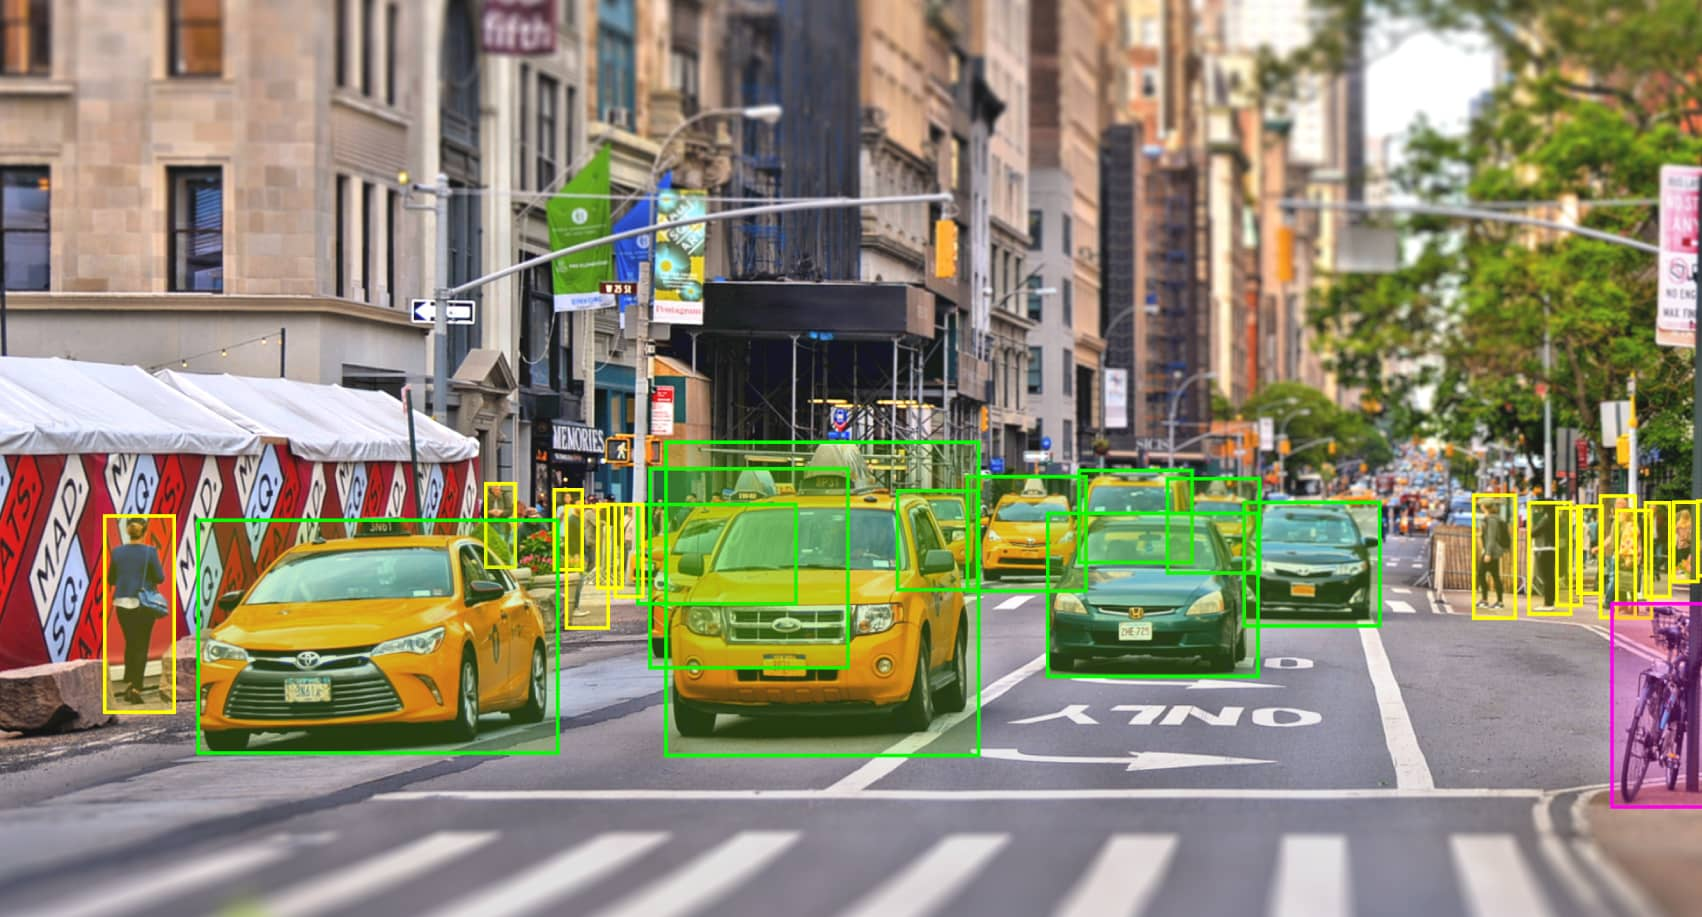
\includegraphics[width=\textwidth]{img/13.jpeg}
				\caption{Illustration d'une annotation de donnée}
			\end{minipage}
		\end{center}
	\end{figure}
	
	
	\subsection{Une ontologie}
	\quad Une ontologie OWL (Web Ontology Language) est une représentation formelle et structurée de connaissances dans un domaine spécifique. OWL est un langage de représentation des connaissances basé sur le Web, utilisé pour décrire les relations entre les concepts dans un domaine donné. Il est principalement utilisé dans le domaine de la gestion des connaissances, de la sémantique web et de l'intelligence artificielle.
	
	Les ontologies OWL sont construites à l'aide de classes, de propriétés et d'individus. Les classes représentent des ensembles de choses ayant des caractéristiques similaires, les propriétés définissent les relations entre les classes et les individus, et les individus représentent des instances spécifiques de classes.
	
	Les ontologies OWL permettent de formaliser les connaissances de manière à ce qu'elles puissent être interprétées par des machines, facilitant ainsi la recherche, la récupération et l'analyse des informations dans divers domaines d'application. Elles sont largement utilisées dans des domaines tels que la bioinformatique, l'ingénierie des connaissances, la gestion des ressources et bien d'autres encore.
	
	\subsubsection{Rapport entre une ontologie et le web sémantique}
	\begin{itemize}
		\item \textbf{Représentation des connaissances :} Les ontologies sont des structures formelles qui définissent des concepts, des relations et des propriétés dans un domaine particulier. Elles permettent de représenter la connaissance d'un domaine de manière précise et structurée. Le Web sémantique fournit un ensemble de standards et de technologies (comme RDF, OWL et SPARQL) pour représenter et échanger ces ontologies sur le Web, permettant ainsi aux machines de comprendre et d'interpréter les données de manière plus intelligente.
		
		\item \textbf{Interopérabilité des données :} En utilisant des ontologies compatibles avec les standards du Web sémantique, il est possible de créer des données interopérables qui peuvent être partagées et intégrées entre différents systèmes et applications. Cela facilite l'échange de données entre les organisations, les domaines de connaissances et les communautés d'utilisateurs.
		
		\item \textbf{Raisonnement automatique :} Les ontologies permettent de définir des axiomes, des règles et des restrictions sur les données et les concepts d'un domaine. Le Web sémantique fournit des langages et des outils pour réaliser du raisonnement automatique sur ces ontologies, permettant ainsi de déduire de nouvelles connaissances à partir des informations existantes.
		
		\item \textbf{Recherche d'information avancée :} En utilisant les ontologies et les technologies du Web sémantique, il est possible d'améliorer la recherche d'information en permettant aux moteurs de recherche de comprendre le sens des données et des requêtes, plutôt que de se contenter de mots-clés. Cela ouvre la voie à des fonctionnalités de recherche plus avancées et plus précises.
		
		\item \textbf{Applications intelligentes :} La combinaison des ontologies et du Web sémantique permet de développer des applications intelligentes qui exploitent les connaissances formelles pour prendre des décisions, recommander des actions et fournir des services personnalisés. Par exemple, les assistants virtuels, les systèmes d'analyse de données et les systèmes d'aide à la décision peuvent bénéficier de cette approche.
	\end{itemize}
	
	\subsection{Outils}
	\subsubsection{Outils de modélisation ontologique}
	Il existe plusieurs outils permettant de créer une ontologie:
	
	\begin{itemize}
		\item \textbf{TopBraid Composer: } Un outil de modélisation des ontologies et de développement d'applications Web sémantiques, offrant des fonctionnalités avancées pour la création et la 
		\item \textbf{Semantic MediaWiki:} Une extension de MediaWiki qui permet d'ajouter des annotations sémantiques aux pages Wiki, facilitant la création de bases de connaissances sémantiques collaboratives.
		\item \textbf{PoolParty:} Une plateforme de gestion des connaissances sémantiques qui permet la création, l'organisation et la publication d'ontologies et de bases de connaissances sémantiques.
		\item \textbf{RDFLib} Une bibliothèque Python pour travailler avec des données RDF, offrant des fonctionnalités pour la création, la manipulation et le stockage de graphes RDF dans des applications Python.
		\item \textbf{Semantic Web Rule Language (SWRL):}
		\item \textbf{GraphDB:} Une base de données de graphes RDF conçue pour stocker et interroger des données RDF à grande échelle, offrant des fonctionnalités avancées pour la gestion des données sémantiques.
		\item \textbf{Protégé:} Protégé est une plateforme de développement open source qui offre des fonctionnalités de modélisation et de gestion des ontologies. Il est largement utilisé dans le domaine de l'intelligence artificielle et du Web sémantique pour créer, éditer et visualiser des ontologies.
	\end{itemize}


	\subsubsection{Choix, intérêts et avantages}
		Choisir \textbf{Protege} comme outil de modélisation et de gestion des ontologies présente plusieurs avantages par rapport à d'autres outils similaires :
		
	
	\begin{table}
		\begin{tabular}{|m{4cm}|m{12cm}|} % Définit deux colonnes de largeur fixe
			\hline
			\textbf{Elements} & \textbf{Descriptions} \\
			\hline
			Large communauté et support actif & Protege est largement utilisé dans la communauté de la recherche en intelligence artificielle et du Web sémantique, ce qui signifie qu'il bénéficie d'une grande communauté d'utilisateurs et de développeurs. Cela garantit un support actif, des forums de discussion animés et une documentation riche. \\
			\hline
			Interface utilisateur conviviale & Protege offre une interface utilisateur conviviale et intuitive qui facilite la modélisation, l'édition et la visualisation des ontologies. Cela le rend accessible même aux utilisateurs débutants dans le domaine de la représentation des connaissances. \\
			\hline
			Fonctionnalités avancées & Protege offre un large éventail de fonctionnalités avancées pour la modélisation et la gestion des ontologies, y compris la validation d'ontologie, le raisonnement automatique, la visualisation graphique des ontologies, la gestion des versions et bien plus encore. \\
			\hline
			Interopérabilité & Protege prend en charge les standards du Web sémantique tels que RDF, OWL et SWRL, ce qui garantit l'interopérabilité avec d'autres outils et systèmes compatibles avec ces standards. Cela facilite l'intégration de Protege dans des pipelines de traitement des connaissances existants. \\
			\hline
			Extensions et plugins & Protege offre un système d'extensions et de plugins qui permet aux utilisateurs d'étendre ses fonctionnalités de base en fonction de leurs besoins spécifiques. Cela permet une personnalisation et une adaptation facile de Protege à divers contextes d'utilisation. \\
			\hline
			Évolution continue & Protege est un projet open source actif qui continue à évoluer et à s'améliorer au fil du temps. Les nouvelles versions sont régulièrement publiées, intégrant des fonctionnalités améliorées, des corrections de bugs et des améliorations de performance. \\
			\hline
		\end{tabular}
		\caption{Avantages de Protege}
		\label{tab:protege_advantages}
	\end{table} 

	\subsection{Les maladies du manioc}
	\quad L'analyse sémantique des images des maladies du manioc est une nouvelle approche pour protéger cette culture importante. Le manioc est essentiel pour de nombreuses communautés dans les régions tropicales, mais il est souvent menacé par des maladies. Dans cette étude, nous examinons comment utiliser des techniques spéciales pour comprendre et détecter les maladies du manioc à partir d'images des feuilles, des tiges ou des racines infectées.
	
	\quad La culture du manioc est confrontée à diverses menaces, notamment des maladies qui peuvent avoir un impact significatif sur la production et la qualité des récoltes. Parmi les maladies les plus préoccupantes\cite{msikita_lutte_nodate}, on trouve : \\ \\
	\textemdash \textbf{  Maladie de la Mosaïque du Manioc, } \\
	\textemdash \textbf{ Maladie de la Tache Brune du Manioc, } \\
	\textemdash \textbf{ Flétrissement Bactérien du Manioc, } \\
	\textemdash \textbf{ Acarien Vert du Manioc, } \\
	\textemdash \textbf{  Pourriture des Racines du Manioc, } \\
	\textemdash \textbf{ Anthracnose du ManiocAnthracnose du Manioc, } \\
	\textemdash \textbf{ Flétrissement Bactérien du Manioc, } \\
	\textemdash \textbf{ Maladie Rose du Manioc, } \\
	\textemdash \textbf{ Nanisme du Manioc } \\
	\textemdash \textbf{ Tache Foliaire du Manioc } \\	
	\textemdash \textbf{ Nématode à Nœuds Radiculaires du Manioc } \\	
	\textemdash \textbf{ Moucheron Blanc du Manioc } \\	
	\textemdash \textbf{ Etc } \\	
	
	Dans cette étude, nous nous concentrerons sur l'analyse sémantique des images pour détecter et comprendre ces maladies spécifiques du manioc.Nous mettrons donc l'accent sur : \\ \\
	\textemdash \textbf{ Brûlure bactérienne (Bacterial Blight (CBB)), } \\
	\textemdash \textbf{ Maladie des stries brunes (Brown Streak Disease (CBSD)), } \\
	\textemdash \textbf{ Marbrure verte (Green Mottle (CGM)), } \\
	\textemdash \textbf{ Maladie de la mosaïque (Mosaic Disease (CMD)) } \\
	
	\subsubsection{Brûlure bactérienne (Bacterial Blight (CBB))}
	\begin{itemize}
		\item \textbf{Images: }
		\begin{figure}[htbp]
			\centering
			\begin{subfigure}[b]{0.3\textwidth}
				\centering
				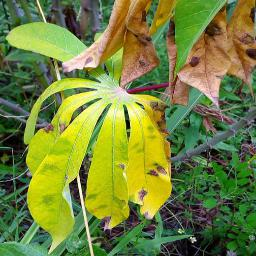
\includegraphics[width=\textwidth]{img/1.jpg}
				\caption{Bactérienne 1}
			\end{subfigure}
			\hfill
			\begin{subfigure}[b]{0.3\textwidth}
				\centering
				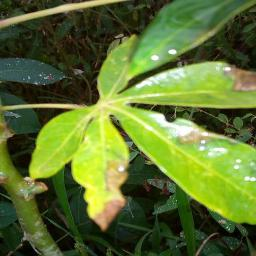
\includegraphics[width=\textwidth]{img/2.jpg}
				\caption{Bactérienne 2}
			\end{subfigure}
			\hfill
			\begin{subfigure}[b]{0.3\textwidth}
				\centering
				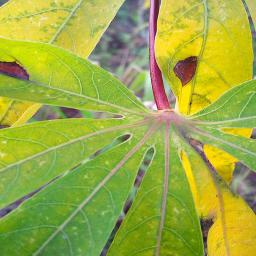
\includegraphics[width=\textwidth]{img/3.jpg}
				\caption{Bactérienne 3}
			\end{subfigure}
			\caption{Images de la brûlure bactérienne}
		\end{figure}
		\item \textbf{Définition: } La brûlure bactérienne est caractérisée par l'apparition de taches nécrotiques, humides et brunes sur les feuilles du manioc. 
		\item \textbf{Cause: } La brûlure bactérienne est une maladie causée par des bactéries qui affectent les plantes, provoquant l'apparition de taches nécrosées sur les feuilles, entraînant souvent le flétrissement, la mort des feuilles et une diminution de la vigueur de la plante.
		\item \textbf{Symptôme: } La bactériose du manioc se présente d'abord sous forme de petites taches humides sur les feuilles, qui deviennent ensuite de plus en plus grandes et brunissent le limbe. Les feuilles touchées finissent par flétrir, mourir et tomber. Ce problème est plus grave pendant la saison des pluies et affecte principalement les jeunes plants.
		\item \textbf{Traitement: } Le traitement de la bactériose du manioc peut impliquer l'utilisation de cultivars résistants, des pratiques culturales appropriées et, parfois, l'application de produits chimiques comme des pesticides.
	\end{itemize}

	\newpage

	\subsubsection{Maladie des stries brunes (Brown Streak Disease (CBSD))}
	\begin{itemize}
		\item \textbf{Images: }
		\begin{figure}[htbp]
			\centering
			\begin{subfigure}[b]{0.3\textwidth}
				\centering
				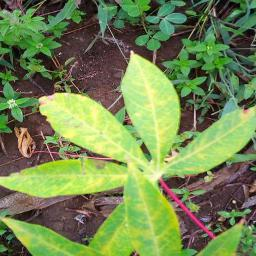
\includegraphics[width=\textwidth]{img/4.jpg}
				\caption{Stries brunes 4}
			\end{subfigure}
			\hfill
			\begin{subfigure}[b]{0.3\textwidth}
				\centering
				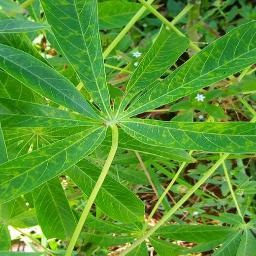
\includegraphics[width=\textwidth]{img/5.jpg}
				\caption{Stries brunes 5}
			\end{subfigure}
			\hfill
			\begin{subfigure}[b]{0.3\textwidth}
				\centering
				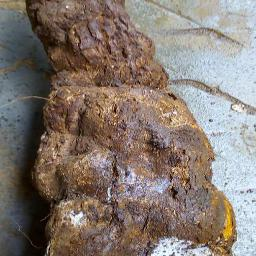
\includegraphics[width=\textwidth]{img/6.jpg}
				\caption{Stries brunes 6}
			\end{subfigure}
			\caption{Images de la maladie des stries brunes}
		\end{figure}
		
		\item \textbf{Définition: } Elle se caractérise par l'apparition de stries brunes sur les racines et les tubercules du manioc infecté, ce qui entraîne une réduction de la qualité et de la quantité des récoltes.
		\item \textbf{Cause: } La Maladie des stries brunes, ou Brown Streak Disease (CBSD), est principalement causée par deux virus du groupe des potyvirus : le virus de la maladie des stries brunes de l'est (BSeMV) et le virus de la maladie des stries brunes de l'ouest (BScMV).
		\item \textbf{Symptôme: } La maladie des stries brunes se manifeste par des symptômes observables sur les feuilles, les tiges et les tubercules du manioc. Sur les feuilles, elle se caractérise par l'apparition de taches jaune-vert, plus prononcées sur les feuilles développées. Contrairement à la mosaïque, les feuilles touchées ne se déforment pas. Sur les tiges, des stries brun foncé ainsi que des lésions nécrotiques peuvent apparaître, principalement sur la partie supérieure verte. Les tubercules peuvent également être déformés, présenter des craquelures et une décoloration.
		\item \textbf{Traitement: } Le traitement de la maladie des stries brunes du manioc peut être difficile car il n'existe pas de méthode curative complètement efficace une fois que la plante est infectée. Cependant, plusieurs approches de gestion peuvent être utilisées pour réduire la propagation de la maladie et limiter ses effets sur les cultures :
		
		\textemdash  Utilisation de cultivars résistants : Sélectionner et cultiver des variétés de manioc qui sont résistantes ou tolérantes à la maladie peut aider à réduire la propagation de la maladie dans les cultures.
		
		\textemdash  Contrôle des vecteurs : La gestion des insectes vecteurs, tels que les pucerons, peut réduire la transmission des virus responsables de la maladie.
		
		\textemdash  Pratiques culturales appropriées : Adopter des pratiques culturales telles que la rotation des cultures, la gestion de l'irrigation et la suppression des plantes infectées peut contribuer à réduire la propagation de la maladie dans les champs.
		
		\textemdash  Utilisation de matériel de plantation sain : Utiliser des boutures de manioc exemptes de maladie pour la plantation peut aider à réduire la propagation de la maladie lors de la multiplication des cultures.
	\end{itemize}

	\newpage

	\subsubsection{Marbrure verte (Green Mottle (CGM))}
	\begin{itemize}
		\item \textbf{Images: }
		\begin{figure}[htbp]
			\centering
			\begin{subfigure}[b]{0.3\textwidth}
				\centering
				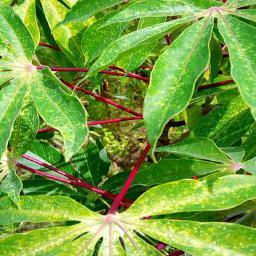
\includegraphics[width=\textwidth]{img/7.jpg}
				\caption{Marbrure verte 7}
			\end{subfigure}
			\hfill
			\begin{subfigure}[b]{0.3\textwidth}
				\centering
				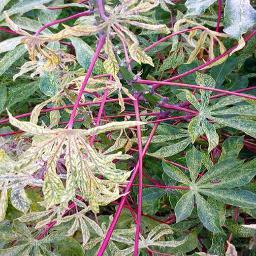
\includegraphics[width=\textwidth]{img/8.jpg}
				\caption{Marbrure verte 8}
			\end{subfigure}
			\hfill
			\begin{subfigure}[b]{0.3\textwidth}
				\centering
				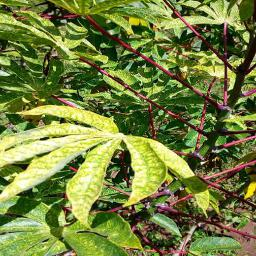
\includegraphics[width=\textwidth]{img/9.jpg}
				\caption{Marbrure verte 9}
			\end{subfigure}
			\caption{Images de la marbrure verte}
		\end{figure}
		
		\item \textbf{Définition: } La Marbrure verte (Green Mottle ou CGM) du manioc se caractérise par l'apparition de marbrures vert clair ou jaune-vert sur les feuilles infectées. Ces marbrures peuvent être irrégulières et s'étendre sur toute la surface des feuilles. Les symptômes sont généralement plus visibles sur la face supérieure des feuilles et peuvent varier en intensité selon le degré d'infection et les conditions environnementales.
		\item \textbf{Cause: } La Marbrure verte (Green Mottle ou CGM) du manioc est principalement causée par une infection virale. Le virus responsable de cette maladie est transmis par des insectes vecteurs, tels que les aleurodes (mouches blanches), qui se nourrissent de la sève des plantes infectées et propagent ainsi le virus à d'autres plantes saines.
		\item \textbf{Symptôme: } Les symptômes de la Marbrure verte (Green Mottle ou CGM) sur les feuilles du manioc se manifestent généralement par l'apparition de marbrures vert clair ou jaune-vert. Ces marbrures peuvent être irrégulières et se propager sur toute la surface des feuilles. Les feuilles affectées peuvent également présenter des déformations et un rabougrissement. Les symptômes peuvent varier en fonction de la gravité de l'infection et des conditions environnementales.
		\item \textbf{Traitement: } Le traitement de la Marbrure verte du manioc (Green Mottle ou CGM) est principalement axé sur la gestion des populations d'insectes vecteurs responsables de la transmission du virus. Voici quelques mesures de gestion qui peuvent être adoptées :
		
		\textemdash  Contrôle des insectes vecteurs : Utilisation de méthodes de lutte intégrée telles que l'utilisation de pièges, de filets anti-insectes et de produits phytosanitaires pour réduire les populations d'insectes vecteurs, comme les aleurodes.
		
		\textemdash  Cultivars résistants : Sélection et plantation de variétés de manioc résistantes ou tolérantes à la maladie, si disponibles.
		
		\textemdash  Rotation des cultures : Pratique consistant à alterner les cultures de manioc avec d'autres cultures non sensibles à la maladie pour réduire la pression des vecteurs et la propagation du virus.
		
		\textemdash  Élimination des plantes infectées : Enlever et détruire les plantes infectées dès l'apparition des symptômes pour réduire la source de l'inoculum viral dans les champs.
	\end{itemize}

	\newpage

	\subsubsection{Maladie de la mosaïque (Mosaic Disease (CMD))}
	\begin{itemize}
		\item \textbf{Images: }
		\begin{figure}[htbp]
			\centering
			\begin{subfigure}[b]{0.3\textwidth}
				\centering
				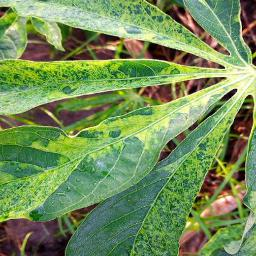
\includegraphics[width=\textwidth]{img/10.jpg}
				\caption{Mosaïque 10}
			\end{subfigure}
			\hfill
			\begin{subfigure}[b]{0.3\textwidth}
				\centering
				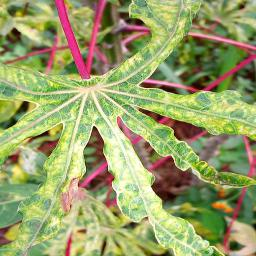
\includegraphics[width=\textwidth]{img/11.jpg}
				\caption{Mosaïque 11}
			\end{subfigure}
			\hfill
			\begin{subfigure}[b]{0.3\textwidth}
				\centering
				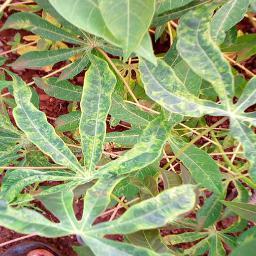
\includegraphics[width=\textwidth]{img/12.jpg}
				\caption{Mosaïque 12}
			\end{subfigure}
			\caption{Images de la maladie de la mosaïque}
		\end{figure}

		\item \textbf{Définition: } La Maladie de la mosaïque du manioc se caractérise par l'apparition de motifs de mosaïque sur les feuilles des plants infectés. Ces motifs se présentent sous forme de zones de couleur verte et jaune irrégulières et distinctes.
		\item \textbf{Cause: } La mosaïque du manioc est causée par un virus
		qui s’introduit dans les feuilles et les tiges du
		manioc.
		\item \textbf{Symptôme: } La Maladie de la mosaïque du manioc est principalement causée par des virus, tels que le virus de la mosaïque du manioc (Cassava Mosaic Virus, CMV) et d'autres virus apparentés du groupe des begomovirus. Ces virus sont transmis par des pucerons vecteurs lorsqu'ils se nourrissent de la sève des plantes infectées.
		\item \textbf{Traitement: } Il n'existe pas de traitement curatif pour la Maladie de la mosaïque du manioc une fois que les plantes sont infectées par le virus. Cependant, plusieurs mesures peuvent être prises pour réduire les risques d'infection et limiter les dommages causés par la maladie :
		
		\textemdash  Utilisation de cultivars résistants : Planter des variétés de manioc qui sont génétiquement résistantes ou tolérantes à la Maladie de la mosaïque du manioc peut aider à réduire la propagation de la maladie dans les cultures.
		
		\textemdash  Contrôle des vecteurs : Mettre en place des mesures de contrôle des pucerons vecteurs, tels que l'utilisation de pièges, de filets anti-insectes et de produits phytosanitaires, peut aider à réduire la transmission du virus.
		
		\textemdash  Pratiques culturales appropriées : Adopter des pratiques culturales telles que la rotation des cultures, la gestion de l'irrigation et l'élimination des mauvaises herbes peut contribuer à réduire la pression des vecteurs et la propagation du virus.
	\end{itemize}

	\section{Chapitre 2 : Mise en place de l'ontologie}
	\subsection{Conceptualisation}
	\quad Dans le cadre d'une ontologie sur la maladie du manioc, nous allons modéliser différents aspects de cette maladie : \textbf{la maladie} , \textbf{les symptômes} , \textbf{les causes} , \textbf{les traitements}.
	
	\begin{enumerate}
		\item \textbf{\large{Classes}}
		\begin{itemize}
			\item MaladieDuManioc
			\item Symptôme
			\item Cause
			\item Traitement
		\end{itemize}
		
		\item \textbf{\large{Propriétés}}
		\begin{itemize}
			\item aPourSymptôme (propriété d'objet entre une maladie du manioc et ses symptômes)
			\item aPourCause (propriété d'objet entre une maladie du manioc et ses causes)
			\item aPourTraitement (propriété d'objet entre une maladie du manioc et ses traitements)
			\item aPourImage (propriété de données entre une maladie du manioc et son image représentative)
		\end{itemize}
		
		\item \textbf{\large{Axiomes}}
		\begin{itemize}
			\item Une maladie du manioc a au moins un symptôme.
			\item Une maladie du manioc a au moins une cause.
			\item Une maladie du manioc a au moins un traitement.
		\end{itemize}
		
		\item \textbf{\large{Instances}}
		\begin{itemize}
			\item MaladieDuManioc : Maladie de la mosaïque, Maladie des stries brunes, Marbrure verte, Brûlure bactérienne
			\item Symptôme : DécolorationDesFeuilles, Nécrose.
			\item Cause : Virus, Bactéries.
			\item Traitement : UtilisationDePesticides, ModificationDuSol, UtilisationDeCultivarsResistants, Contrôle des vecteurs
		\end{itemize}

	\end{enumerate}

	\newpage
	\section{Bibliographies}
	
	\bibliographystyle{plain} % Style de la bibliographie
	\bibliography{c} % Nom du fichier .bib (sans l'extension)
	%\bibliographystyle{smfplain}
	
\end{document}
